\documentclass[a4paper, oneside]{article}
\usepackage{array}
\usepackage{shortvrb}
\usepackage{listings}
\usepackage{fullpage}
\usepackage{enumerate}
\usepackage{graphicx}
\usepackage{subfigure}
\usepackage{url}
\usepackage{indentfirst}
\usepackage{eurosym}
\usepackage{listings}
\usepackage{color}
\usepackage{fancybox}
\usepackage{ulem}
\usepackage{wrapfig}
\usepackage{systeme}
\usepackage{tabularx}
\usepackage{subfig}
\usepackage[dvipsnames]{xcolor}



\begin{document}
\begin{titlepage}
	\newcommand{\HRule}{\rule{\linewidth}{0.5mm}}
	\center
	\textsc{\LARGE Université de Liège}\\[1cm]
	\textsc{\Large Faculté des Sciences Appliquées}\\[2cm]
		
	\HRule \\[0.5cm]
	{ \huge \bfseries Automatic Multispeaker Voice Cloning Across Languages}\\[0.2cm]
	\HRule \\[3cm]

	\begin{minipage}{0.4\textwidth}
		\begin{flushleft} \Large
			\emph{Author:}\\
			Corentin \textsc{Jemine}
		\end{flushleft}
	\end{minipage}
	~
	\begin{minipage}{0.4\textwidth}
		\begin{flushright} \Large
			\emph{Supervisor:} \\
			Prof. Gilles \textsc{Louppe}
		\end{flushright}
	\end{minipage}\\[4cm]
	
	{\LARGE Academic year 2018 - 2019}\\[2cm]
	
	
\includegraphics{images/uliege_logo.jpg}\\[1.25cm]
	
	\textit{Graduation studies conducted for obtaining the Master's degree \\in Data Science by Corentin Jemine}
	
	\vfill
\end{titlepage}

\setcounter{page}{2}

\color{red}
Possibly, start with a TTS lexicon with some definitions. Meanwhile, I'll make a list of TSS-specific words that may be worth explaining: coarticulation, linguistic context, rich context, spectral envelope, fundamental frequency, supra-segmental
\color{black}

\section{Abstract}
\color{red}
To do when I'll have a good overview of the project. Try to answer:
\begin{itemize}
	\item What is the goal of the application? What are its requirements, what is the setting, what kind of data are we going to use it on?
	\item What is zero-shot voice cloning? How does it fit in here (difference between an online and offline approach)?
	\item What are the particularities of our implementation (both model and datasets), what are its upsides and downsides (for example: requires huge datasets but fast inference)?
	\item What did we ultimately achieve? How good are our results?
\end{itemize}
\color{black}

\section{Introduction}

\color{red}
Concise presentation of the problem
\color{black}


\subsection{Statistical parametric speech synthesis}
Statistical parametric speech synthesis (SPSS) refers to a group of data-driven TTS synthesis methods that emerged in the late 1990s. In SPSS, the relation between features computed on the input text and output acoustic features is modeled by a statistical generative model (called the acoustic model). A complete SPSS framework thus also includes a pipeline to extract features from the text to synthesize as well as a system able to reconstruct an audio waveform from the acoustic features produced by the acoustic model (such a system is called a vocoder). Unlike the acoustic model, these two parts of the framework may be entirely engineered and make use of no statistical methods. If it is possible to condition parts of the framework in such a way that the characteristics of the generated voice are modified, then the framework is a multispeaker TTS synthesis system.

The processing of text into features can be nearly inexistent as it can be very extensive. Speech is an intricate process that depends on a wide range of linguistic contexts. Providing these contexts greatly reduces the extent of the task to be learned by the acoustic model, but may require complex natural language processing (NLP) techniques or accuracy trade-offs, especially for rare or unknown words. Linguistic contexts are retrieved on different levels: utterance, phoneme, syllable, word and phrase. For each of those elements, their neighbouring elements of the same level are usually considered, as well as the elements lower in the hierarchy it comprises. For example, a given frame will contain a word, the two previous words, the two following words and the syllables contained in all those words. The position of each element with regard to its parent element can be included (e.g. fifth word in a sentence), as well as grammatical information such as part of speech. For syllables, the lexical stress and accent can be predicted by a statistical model such as a decision tree. For prosody, ToBI \cite{TOBI} is often used.

\color{red}Talk about evaluation metrics (mainly MOS)?\color{black}

\subsection{State of the art in multispeaker TTS}
Previous state of the art in SPSS includes hidden Markov models (HMM) based speech synthesis \cite{Tokuda-2013}. The speech generation pipeline is laid out in figure \ref{hmm_spss_framework}. In this framework, the acoustic model is a set of HMMs. The input features are rich linguistic contexts. Ideally, one would train an HMM for each possible context; but as the number of contexts increases exponentially with the number of factors considered, it is not practical to do so. Indeed, not every context will be found in a typical dataset and the training set would then be partitioned over the different contexts, which is very data inefficient. Instead, contexts are clustered using decision trees and an HMM is learned for each cluster \cite{HMMTTS}. Note that this does not solve entirely the training set fragmentation problem. The HMMs are trained to produce a distribution over mel-frequency cepstral coefficients (MFCC) with energy (called static features), their delta and delta-delta coefficients (called dynamic features), as shown in figure \ref{mlpg_features}. A new sequence of static features is retrieved from these static and dynamic features using the maximum likelihood parameter generation (MLPG) algorithm \cite{Tokuda-2000}. These static features are then fed through the MLSA \cite{MLSA} vocoder. 

It is possible to modify the voice generated by conditioning on a speaker or tuning the generated speech parameters with adaptation or interpolation techniques (e.g. \cite{HMMSpeakerInterpolation}  \color{red} elaborate a bit on these techniques?\color{black}), making HMM-based speech synthesis a multispeaker TTS system. \color{red} Compare with concatenative see \cite{SPSSDNN} and https://ieeexplore.ieee.org/document/541110.\color{black}

\begin{figure}[h]
	\centering
	\begin{minipage}{.45\linewidth}
		\centering
		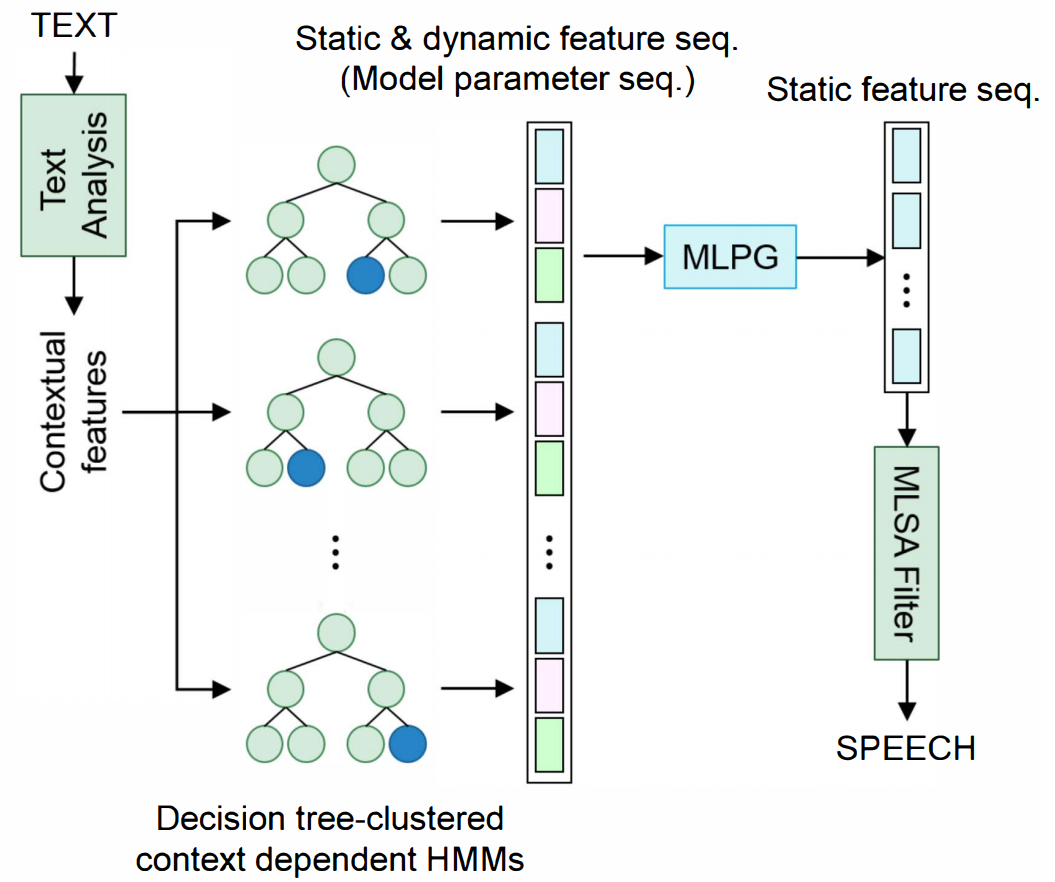
\includegraphics[width=\linewidth]{images/hmm_spss.png}
		\captionof{figure}{The general HMM-based TTS synthesis approach.}
		\label{hmm_spss_framework}
	\end{minipage}
	\hspace{.05\linewidth}
	\begin{minipage}{.45\linewidth}
		\centering
		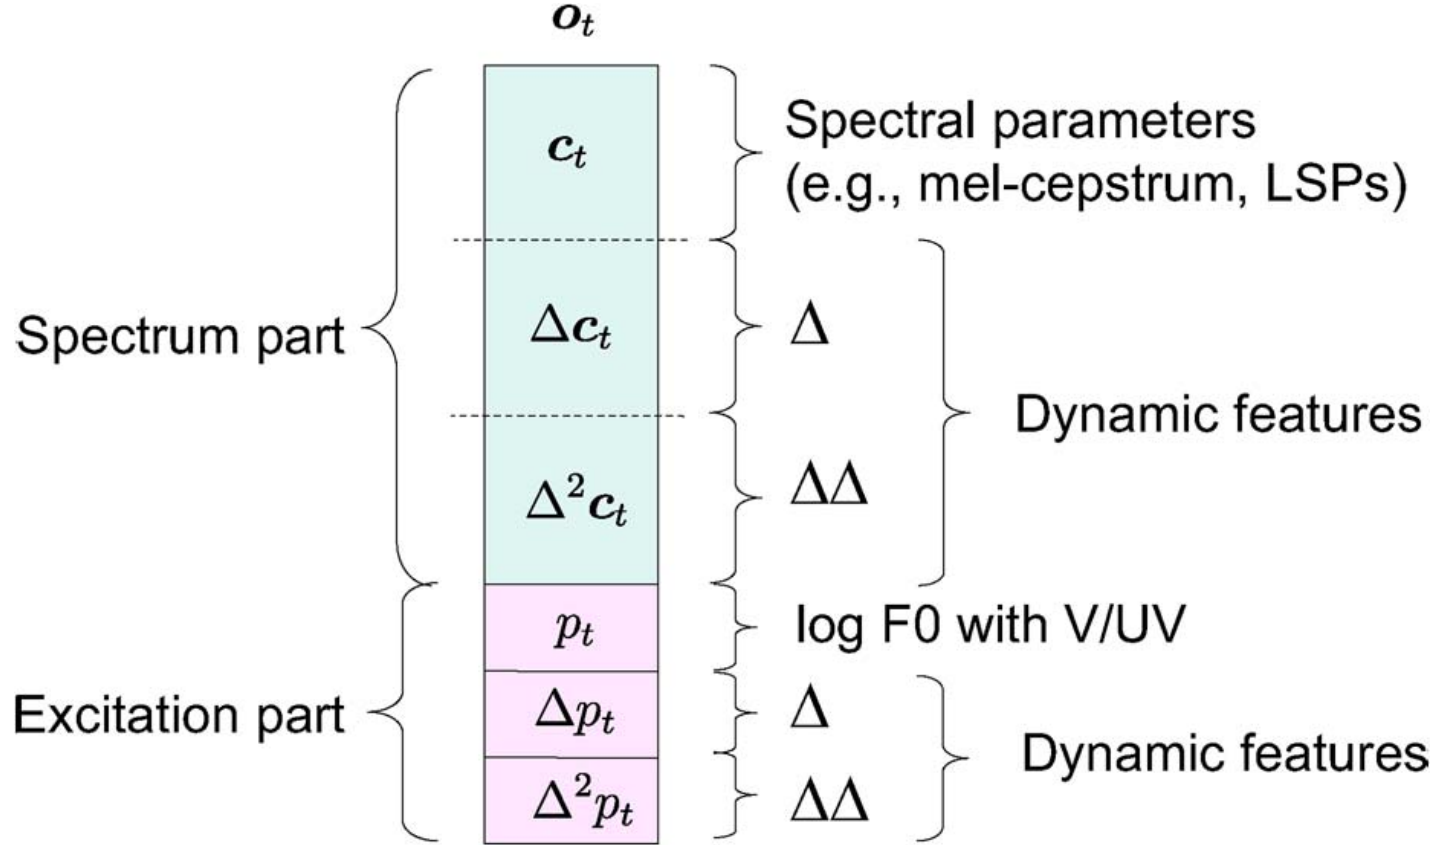
\includegraphics[width=\linewidth]{images/mlpg_features.png}
		\captionof{figure}{Dynamic and static features produced by the HMMs}
		\label{mlpg_features}
	\end{minipage}
\end{figure}

Improvements to this framework were later brought by feed-forward and recurrent deep neural networks (DNN and RNN respectively), as a result of progress in both hardware and software. \cite{SPSSDNN} proposes to replace entirely the decision tree-clustered HMMs in favor of a DNN. They argue for better data efficiency as the training set is no longer fragmented in different clusters of contexts\color{red}, and for a more powerful model?\color{black}. They demonstrate improvements over the speech quality with a number of parameters similar to that of the HMM-based approach. Their best model is a DNN with 4 layers of 256 units using a sigmoid activation function. Subjects assessing the quality of the generated audio samples report that the DNN-based models produces speech that sounds less muffled than that of the HMM-based models. Later researches corroborate these findings \cite{OnTheTrainingAspects}. \cite{Hashimoto-2015} additionally studies the effect of replacing MLPG with another DNN. The combinations of HMM/DNN and MLPG/DNN give rise to four possible frameworks, the novel ones being HMM+DNN and DNN+DNN\footnote{Note that since the two networks are consecutive in the framework, they can be considered as a single network.}, while HMM+MLPG and DNN+MLPG are respectively the frameworks described in \cite{Tokuda-2013} and \cite{SPSSDNN}. Each DNN they used is 3 layers deep with 1024 units using a sigmoid activation function. The MOS of each combination is reported in figure \ref{hashimoto_results}. \color{red} How much do we care about their results? Should I make this part shorter? How about a table at the end that groups all MOS \color{black}

%\begin{wraptable}{r}{5.5cm}
%	\begin{tabular}{| l | c |}
%		\hline
%		Method & MOS \\
%		\hline
%		HMM+MLPG & 3.08 ($\pm$0.12) \\
%		HMM+DNN & 2.86 ($\pm$0.12) \\
%		\textbf{DNN+MLPG} & \textbf{3.53 ($\pm$0.12}) \\
%		DNN+DNN & 3.17 ($\pm$0.12) \\
%		\hline
%	\end{tabular}
%	\caption{MOS of the different methods explored in \cite{Hashimoto-2015}}
%	\label{hashimoto_results}
%\end{wraptable}


\color{red}
Also read \cite{Yin2014ModelingDP}
\color{black}


\color{red}


Wavenet: breakthrough in TTS with raw waveform gen

Take images from https://deepmind.com/blog/wavenet-generative-model-raw-audio/ ?

Dilated causal convolutions

Condition on a speaker identity

Tacotron

Deep voice (1, 2, 3 + few samples), Tacotron 2

SV2TTS

Extensions?
\color{black}



\color{red}
\color{black}

\clearpage
\bibliographystyle{plain}
\bibliography{references} 




















%$$\Leftrightarrow h_b(x) =
%\left\{\begin{array}{lll}
%0 & if & P(y = 0 | x) > P(y = 1 | x)\\ 
%1 & else &
%\end{array}\right.$$



%\begin{figure}[h]
%	\centering
%	\includegraphics[width=16cm]{image.png}
%	\caption{caption}
%	\label{label}
%\end{figure}



%\begin{figure}[h]
%	\centering
%	\captionsetup{justification=centering}
%	\hspace{-1cm}
%	\subfigure{\includegraphics[height=5cm]{image.png}}
%	\subfigure{\includegraphics[height=5cm]{image.png}}
%	\hspace{-1cm}
%	\caption{caption}
%	\label{label}
%\end{figure}


%\begin{center}
%	\begin{tabular}{|r|ccc|ccc|}
%		\hline
%		& \multicolumn{6}{c|}{Validation set}\\
%		\hline
%		& \multicolumn{3}{c|}{Valid images (3126)} & \multicolumn{3}{c|}{Invalid images (3126)} \\
%		\hline
%		& Correct & Unclassified & Incorrect & Correct & Unclassified & Incorrect \\
%		\hline
%		Reduced & 94.98\% & 3.07\% & 1.95\% & 95.27\% & 2.91\% & 1.82\% \\
%		Lenet & 98.08\% & 0.74\% & 1.18\% & 97.86\% & 0.96\% & 1.18\% \\
%		\hline
%	\end{tabular}
%	
%	\vspace{0.5cm}
%	  
%	\begin{tabular}{|r|ccc|ccc|}
%		\hline
%		& \multicolumn{6}{c|}{Test set}\\
%		\hline
%		& \multicolumn{3}{c|}{Valid images (999)} & \multicolumn{3}{c|}{Invalid images (74)} \\
%		\hline
%		& Correct & Unclassified & Incorrect & Correct & Unclassified & Incorrect \\
%		\hline
%		Reduced& 94.29\% & 3.70\% & 2.00\% & 95.95\% & 4.05\% & 0.00\%  \\
%		Lenet & 96.90\% & 1.30\% & 1.80\% & 97.30\% & 1.35\% & 1.35\% \\
%		\hline
%	\end{tabular}
%\end{center}


\end{document}













































































































